


\begin{figure}[t]
	\centering
	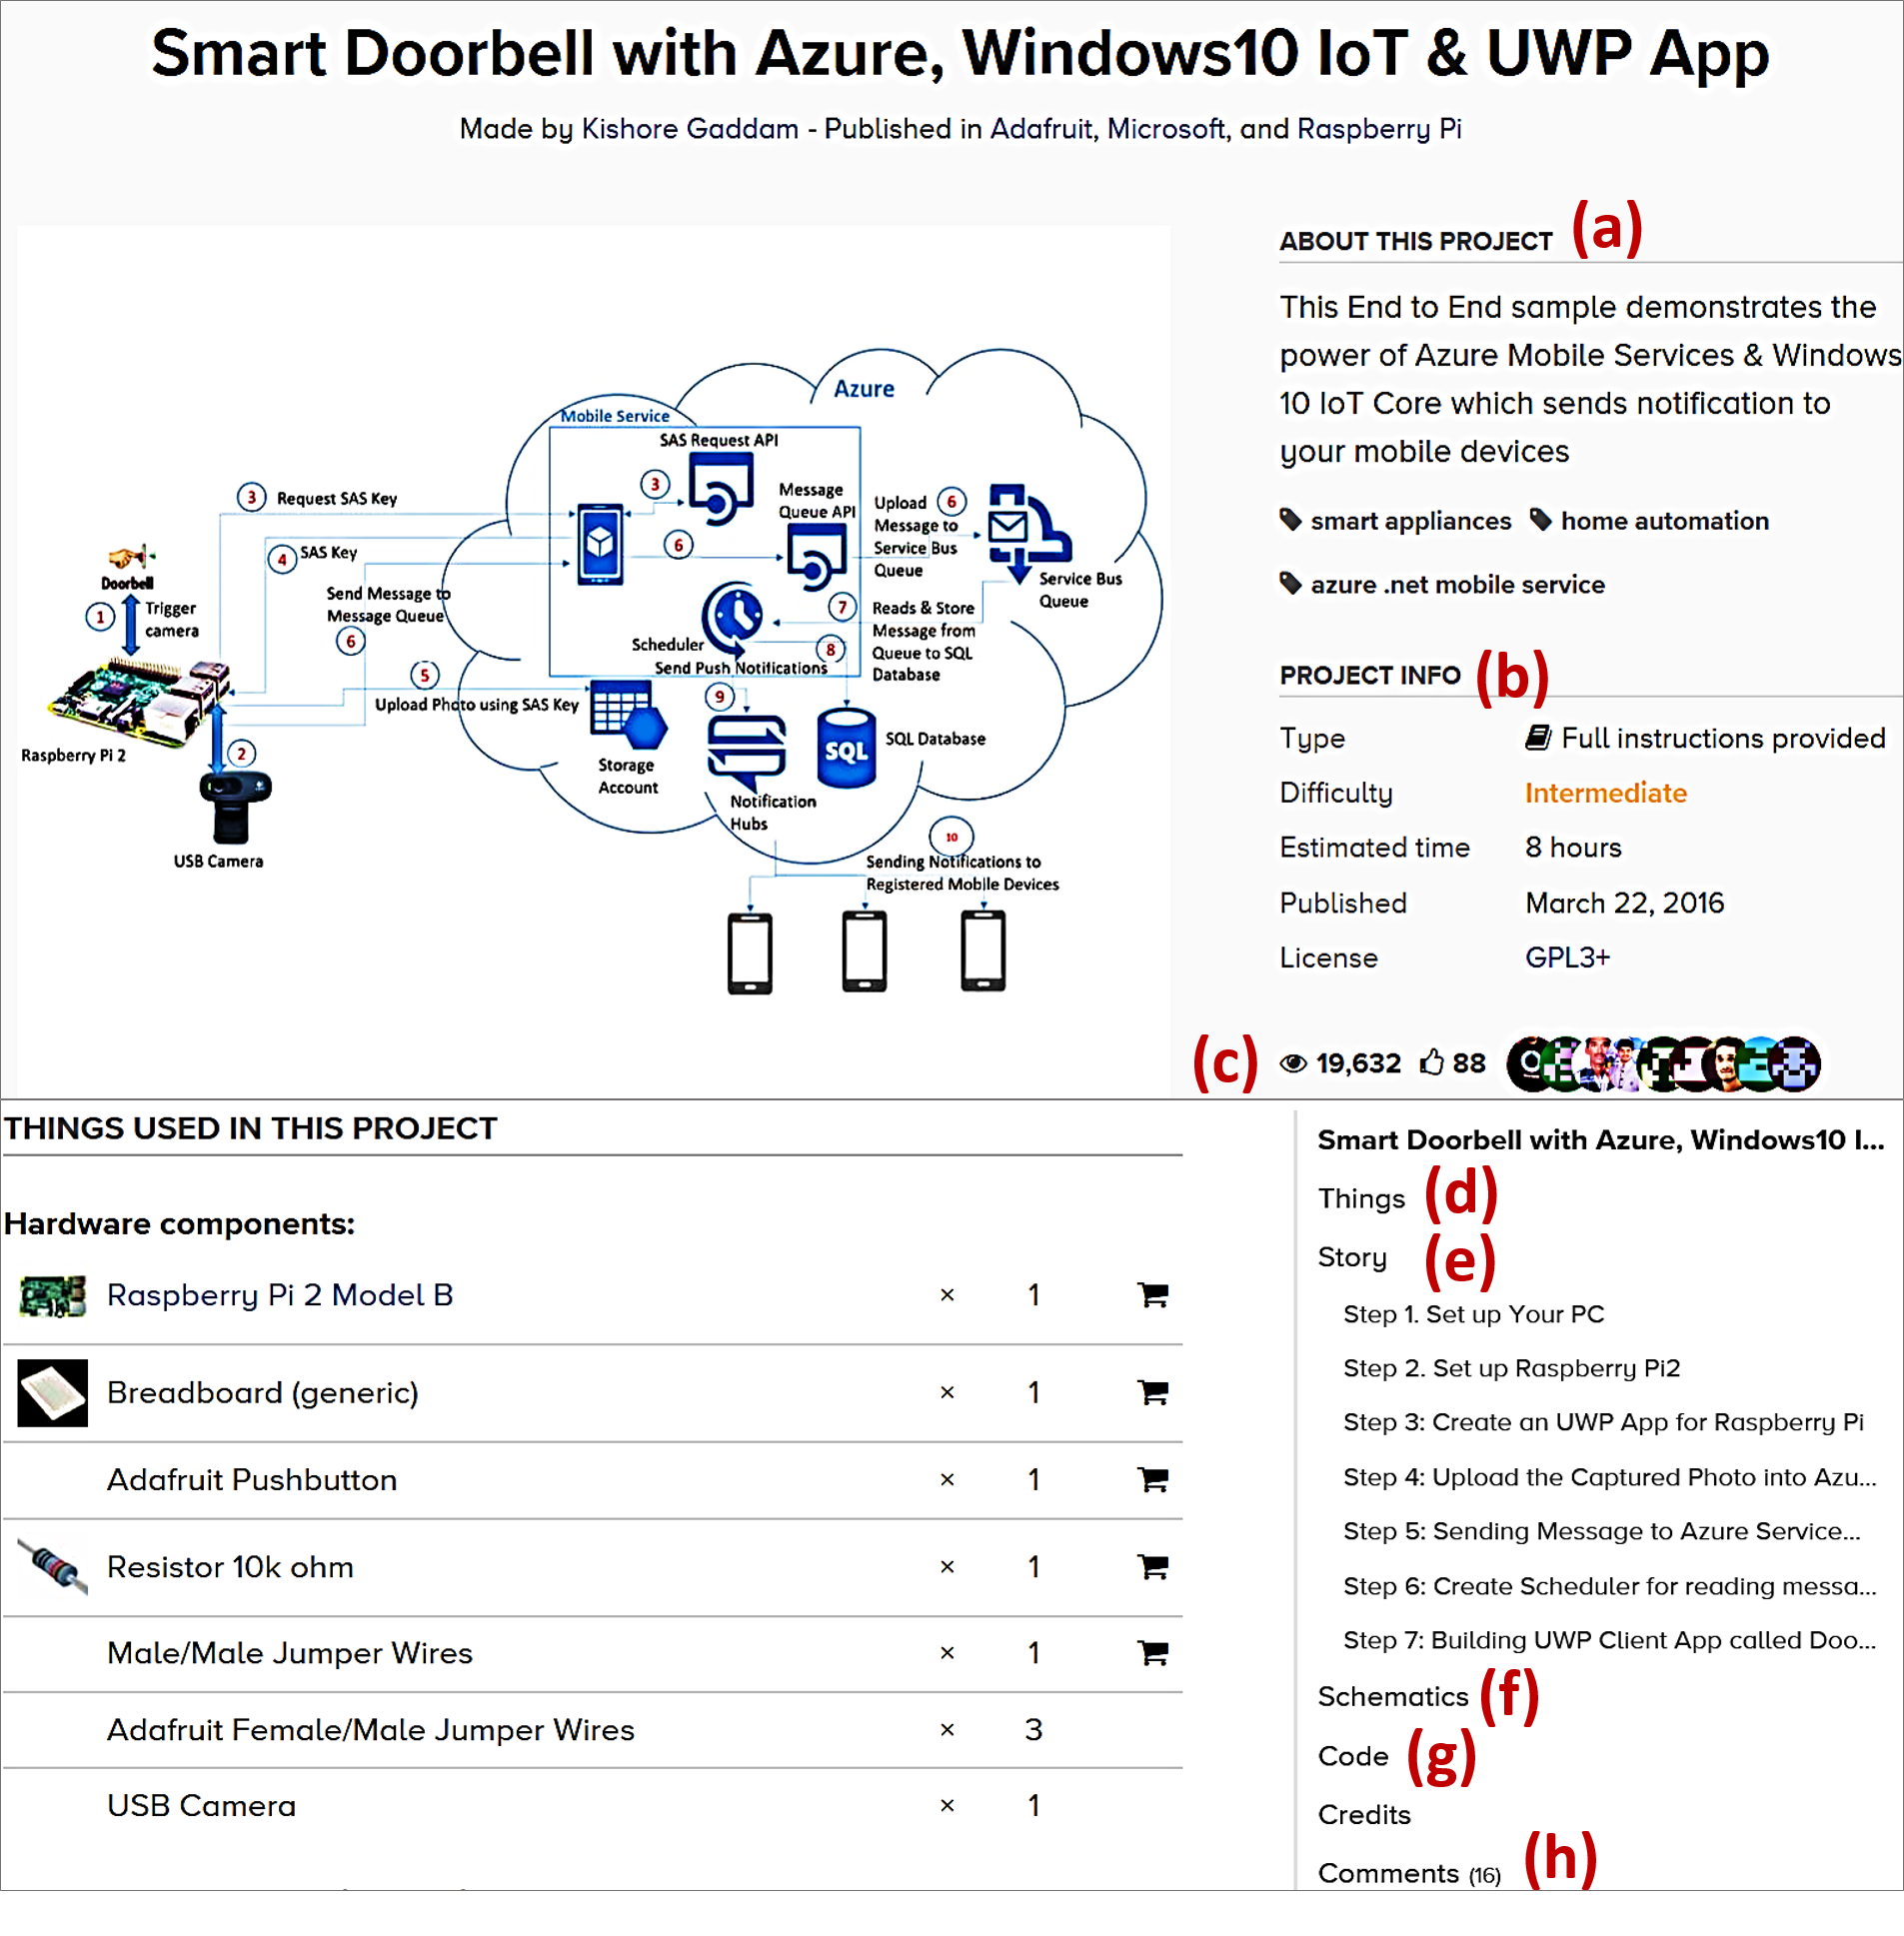
\includegraphics[width=8cm]
	{Figures/hackster05.png}
%	\vspace{-0.1cm}
	\caption {An example of a project on the Hackster, including: (a) project description and tags, (b) basic project information, (c) project view count (the eye icon) and respect count (the thumbs-up icon), (d) hardware and software tools, (e) stories, (f) schematics, (g) source-code, and (h) user comments.}
	\label{hacksterproject}	
	\vspace{-0.2cm}
\end{figure}


\section{Data Collection}\label{datacol}

In this section, we briefly describe the documents that we retrieve to measure the required metrics. The primary sources are the Hackster~\cite{hackster} and the GitHub~\cite{github}.
For each project, we retrieve the associated source-code either from the \textit{GitHub} (888 projects) using the link that is provided on the project page, or directly from the Hackster (344 projects) if applicable.

\textit{Hackster}~\cite{hackster} is one of the largest and the most active IoT development communities.
As of $October\ 2017$, the Hackster has over $290,000$ registered users and more than $65\%$ of them are professional engineers.
Over $5,000$ active IoT projects are currently managed on the Hackster~\cite{hackster}.

\textit{GitHub} is a version control repository and hosting service that offers various functionalities, such as source-code management~\cite{github}.

We study the IoT projects that are based on the \textit{Raspberry} and \textit{Arduino} platforms, i.e., the two most popular IoT hardware platforms~\cite{iotanalytics,hackster-survey-2016}.
In total, we collect $855$ Arduino projects and $377$ Raspberry projects from the Hackster that are associated with source-code. Considering source-code allows us to investigate the contribution of the source-code group of metrics to project popularity in comparison with other groups, such as the project page group of metrics.
For each project, we crawl the following documents from the Hackster:

\begin{enumerate}
	\item[(i)] \textit{Project Page}: The project page of an IoT project contains information about the project, such as project description, and development instructions. Figure~\ref{hacksterproject} shows a screen-shot of a sample project on the Hackster.
	\item[(ii)] \textit{User Comments}: Each project on the Hackster can receive comments from users. The comments are available via a link on the project pages.
	%An example of user comments can be found at \href{https://www.hackster.io/cyborg-titanium-14/home-automation-system-using-raspberry-pi-784235#comments}{here}.
	\item[(iii)] \textit{Developer Profile}: Each developer can hold a profile on the Hackster. A developer profile contains information about the developer, such as a brief biography and a list of skills.
	%A sample developer profile can be found at \href{https://www.hackster.io/cyborg-titanium-14}{here}.
	\item[(iv)] \textit{Developer Activities}: Activities of each developer are recorded on the Hackster since joining the Hackster, such as posting comments on other projects.
	%An example of developer activities can be found at \href{https://www.hackster.io/cyborg-titanium-14/activity}{here}.
\end{enumerate}



